\section{Métodologia de pruebas} 
\input{./chapters/031_MétodologiaPruebas.tex}

\section{Infraestructura de pruebas} 
Como entorno de pruebas para la ejecución de los análisis de código; haremos uso de una máquina física y de un contenedor 
de Docker con la siguientes características y herramientas instaladas en cada una de ellas:

\begin{table}[h!]
    \begin{center}
      \caption{Parámetros línea comandos dependency-check}
      \label{tab:Infraestructura de pruebas}
      \begin{tabular}{c|c|c}
        \textbf{Características} & \textbf{Máquina física} & \textbf{Contenedor}\\
        \hline
        Sistema Operativo & Windows 10 Pro & Debian GNU/Linux 10 (buster)\\ 
        Herramientas & OWASP Zap 2.10
        Dependency-check
        SonarScaner 4.6.2
         & SonarQube 8.2
         PostGresSQL 13.3 \\ 
      \end{tabular}
    \end{center}
  \end{table}

Para levantar el contenedor podemos hacer uso de dockercompose incluido en la carpeta \textbf{"entornoPrueba"} dentro de 
las \href{https://github.com/M0l1n3ta/PFG/tree/master}{fuentes de proyecto}

Para levantar el entorno ejecutamos:

\begin{verbatim}
    docker-compose up
\end{verbatim}

\begin{figure}[h!]  
    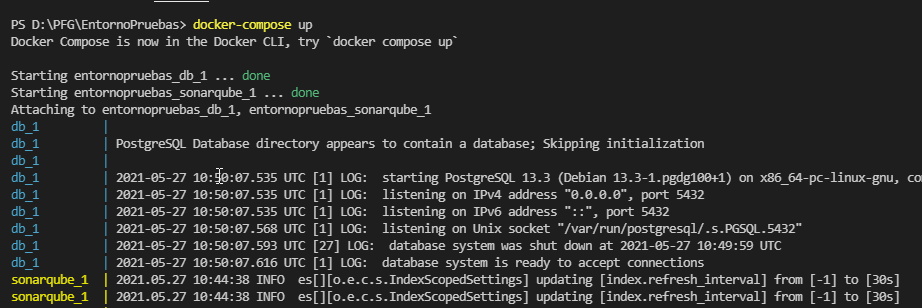
\includegraphics[width=\linewidth]{./imagenes/04_DockerCompose_UP.png}
    \caption{Docker compose up}  
    \label{fig:19}
\end{figure}

Una vez que se vena las siguientes líneas en el log:
\begin{figure}[h!]  
    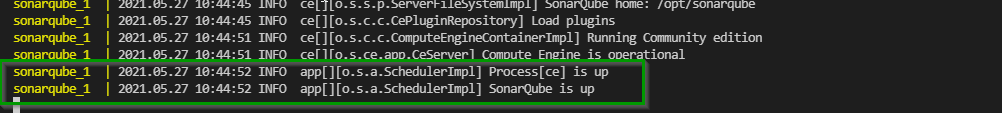
\includegraphics[width=\linewidth]{./imagenes/05_SonarQubeServerRunning.png}
    \caption{SonarQube server running}  
    \label{fig:20}
\end{figure}
Podremos acceder a la página de SonarQube en 
la url \href{http://localhost:9000}{http://localhost:9000}\\
\begin{figure}[h!]  
    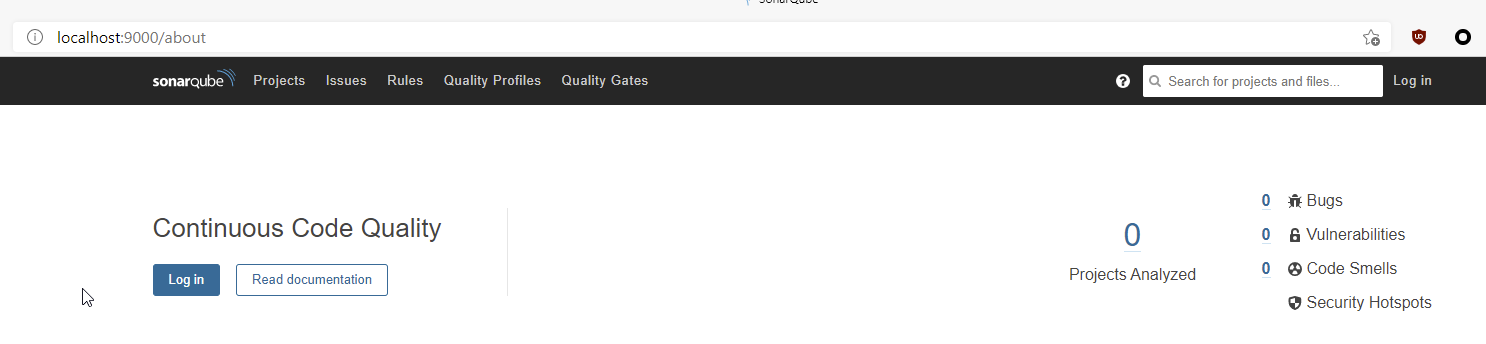
\includegraphics[width=\linewidth]{./imagenes/06_SonarQubeServer_Webpage.png}
    \caption{SonarQube portal}  
    \label{fig:21}
\end{figure}

Docker Compose SonarQube:\\
\begin{listing}[h!]
    \inputminted{yaml}{./EntornoPruebas/SonarQube_8.2/docker-compose.yml}
    \caption{Docker Compose}
    \label{listing:3}
\end{listing}